\documentclass[
    a4paper, aps, twocolumn, floatfix, superscriptaddress,
    nofootinbib]{revtex4-1}

% It's nice to be able to write your own name
\usepackage[T1]{fontenc}
% Automatic clickable links
\usepackage{hyperref}
% SI-units
\usepackage{siunitx}
% Enhanced math formatting
\usepackage{amsmath}
% Extended math symbols
\usepackage{amssymb}
% Include proof environment
\usepackage{amsthm}
\usepackage{enumerate}
% Import the tensor package for tensors
\usepackage{tensor}
% Include dod and dpd fracs
\usepackage{commath}
% Include font for the identity operator
\usepackage{dsfont}
% Include Tikz
\usepackage{tikz}
% Tikz add-on
\usetikzlibrary{shapes,arrows}
\usetikzlibrary{positioning}
% Several figures in the same figure
\usepackage{subfig}
% Appendix
\usepackage[toc, page]{appendix}
\usepackage{simpler-wick}
% Code listings
\usepackage{listings, lstautogobble}
\usepackage{minted}
% Colors
\usepackage{xcolor}
% Directory tree package
\usepackage{dirtree, varwidth}
% Multirow (for table)
\usepackage{multirow}

\usepackage{fontspec}
\newfontfamily\DejaSans{DejaVu Sans}

\newcommand{\nan}{{\DejaSans 😱}}

% Macro for latin-letter vectors
\newcommand{\vf}{\mathbf}
% Macro for greek-letter vectors
\newcommand{\vfg}{\boldsymbol}

% Fast macro for real-numbers R
\newcommand{\R}{\mathbb{R}}
% Fast macro for complex-numbers C
\newcommand{\C}{\mathbb{C}}
% Fast macro for polynomial room P
\renewcommand{\P}{\mathbb{P}}
% New command for the identity operator
\newcommand{\1}{\mathds{1}}
% New command for the Lagrangian density
\newcommand{\cL}{\mathcal{L}}
% New command for the Hamiltonian density
\newcommand{\cH}{\mathcal{H}}
% Fast macro for partial differential tensors
\newcommand{\tpl}[1]{\tensor{\partial}{_#1}} % Lower
\newcommand{\tpu}[1]{\tensor{\partial}{^#1}} % Upper
% Fast macro for tensors
\newcommand{\te}[1]{\tensor{#1}}
% Fast macro for commutation and anti-commutation relations
\newcommand{\com}[2]{\left[#1, #2\right]}
\newcommand{\acom}[2]{\left\{#1, #2\right\}}

% Macros for writing auto-sized paranthesis, brackets and braces
\newcommand{\para}[1]{\left(#1\right)}
\newcommand{\brak}[1]{\left[#1\right]}
\newcommand{\brac}[1]{\left\{#1\right\}}

% Macro for creating orbital bra-ket's, i.e., bra-ket with paranthesis edges
\newcommand{\obra}[1]{( #1 \lvert}
\newcommand{\oket}[1]{\rvert #1 )}
\newcommand{\obraket}[2]{( #1 \lvert #2 )}

% Macro for expectation value
\newcommand{\expv}[1]{\langle #1 \rangle}

\newcommand{\half}{\frac{1}{2}}

\newcommand{\bra}[1]{\langle #1\lvert}
\newcommand{\ket}[1]{\rvert #1\rangle}
\newcommand{\braket}[2]{\langle #1 \vert #2 \rangle}

\newcommand{\acr}[1]{a_{#1}^{\dagger}}
\newcommand{\ade}[1]{a_{#1}}

\newcommand{\kslat}{\ket{\Phi_0}}
\newcommand{\bslat}{\bra{\Phi_0}}

\newcommand{\kcc}{\ket{\Psi_{\text{CC}}}}
\newcommand{\bcc}{\bra{\Psi_{\text{CC}}}}

\newcommand{\ecc}{E_{\text{CC}}}
\newcommand{\eccd}{E_{\text{CCD}}}

% Defining color
\definecolor{light-gray}{gray}{0.9}

% Bash language specifier
\lstnewenvironment{bash}
{\lstset{
    basicstyle=\small\ttfamily, language=bash, keywordstyle=\color{blue},
    backgroundcolor=\color{light-gray}, showstringspaces=false,
    frame=single, autogobble=true, morekeywords={make, git},
    alsoletter={.}}}
{}

\begin{document}

\title{Ground state energy of quantum dots using the coupled cluster method}
\author{Winther-Larsen, Sebastian Gregorius}
\homepage[Project code: ]{https://github.com/Schoyen/FYS4411}
\affiliation{University of Oslo}
\author{Schøyen, Øyvind Sigmundson}
\homepage[Project code: ]{https://github.com/Schoyen/FYS4411}
\affiliation{University of Oslo}
\date{\today}

\begin{abstract}
    The coupled cluster method for estimating the ground state energy of a
    many-body system is arguably the most important post-Hartree-Fock method. We
    have implemented the coupled cluster method with double excitations (CCD).
    We find that it does not perform well with a simple harmonic oscillator
    basis, but the results vastly improve when it is provided a basis from a
    restricted Hatree-Fock self-consistent field method run as a preliminary
    computation. For a system consisting of $N=2$ interacting particles, using
    12 orbital shells we get a ground stated energy of $3.005970$, very close to
    the analytical ``true answer'' of $3$\cite{taut1994two}.
\end{abstract}

\maketitle
\tableofcontents

% FIXME: Replace the two-body matrix elements in bra-ket notation with u-tensor.

\section{Introduction}
    In this project we will compute the ground state energy of quantum dots, a
    construct that has become a popular area of study in recent decades, both
    from a theoretical and an experimental point of view. We achieve the ground
    state computation by implementing a coupled cluster amplitude equation
    solver which is used in succession with a restricted Hartree-Fock
    self-consistent field method.

    Regardless of how sophisticated the method used, the many-body problem
    remains quite intractable. The true wavefunction of any system will be a
    linear combination of all possible slater-type orbitals one can model. This
    means that in order to represent a system correctly, one would need a basis
    set of infinite size. This is an obvious problem when we solve problems
    numerically, because we obviously need to limit the size of the basis we use
    because we have limitations in memeory and computating power. Luckily, great
    minds have bestowed a wide selection of very god numerical methods upon the
    world, which the coupled cluster is a part of.

    First, we provide a thorough theoretical outline of how we model a quantum
    dot, the mathematical formalism behind many-body problems and outline how
    the computational methods we employ both turn into iterative schemes that
    are easy to represent numerically. Second, we provide a brief overview of
    the program we have constructed which is in the form an installable python
    package.  Third, we have employed the methods on a large parameter space
    presenting results for systems consisting of $N= \{2, 6, 12, 20\}$
    particles. Fourth, we discuss the most interesting aspects of the results
    and try to shed some light over the shortcomings as well as the beneficial
    features of the different metods. Lastly, we end on some summary remarks.

\section{Theory}
    In this project we will study a system of $N$ interacting electrons. We will
    be looking at a Hamiltonian consisting of a one-body and a two-body part.
    The one-body part is given by
    \begin{align}
        h(\vf{r}_i)
        &= -\half\nabla_i^2 + \half\omega^2 \vf{r}_i^2,
        \label{eq:one_body_hamiltonian}
    \end{align}
    where we use natural units $\hbar = c = e = 1$ and set the mass to unity.
    % Why not write $\hbar = c = e = m = 1$?
    The two-body part is the Coulomb interaction potential,
    \begin{align}
        u(\vf{r}_i, \vf{r}_j)
        &= \frac{1}{\abs{\vf{r}_i - \vf{r}_j}}.
        \label{eq:two_body_operator}
    \end{align}
    We thus get the total Hamiltonian
    \begin{align}
        H &= h + u
        =
        \sum_{i = 1}^N h(\vf{r}_i) + \sum_{i < j}^N u(\vf{r}_i, \vf{r}_j),
    \end{align}
    where $h$ is the full one-body operator and $u$ the full two-body
    operator, i.e., over the entire system.  Working in a basis of $L$ single
    particle functions, $\{\ket{p}\}_{p = 1}^L$. We define the reference Slater
    determinant as
    \begin{align}
        \ket{\Phi_0} &\equiv \ket{1, 2, \dots, N},
    \end{align}
    i.e., a tensorproduct of the $N$ first single particle functions, $\ket{i}$,
    of the system. We call these single particle functions \emph{occupied} as
    they are contained in the Slater determinant.  We will denote the occupied
    indices with $i, j, k, l, \dots \in \{1, \dots, N\}$, the \emph{virtual}
    states with $a, b, c, d, \dots \in \{N + 1, \dots, L\}$ and general indices
    with $p, q, r, s, \dots \in \{1, \dots, L\}$. In terms of sets of basis
    functions we can write this as
    \begin{align}
        \{\ket{p}\}_{p = 1}^L
        = \{\ket{i}\}_{i = 1}^N
        \cup
        \{\ket{a}\}_{a = N + 1}^L,
    \end{align}
    i.e., the general indexed states consists of both occupied and virtual
    states. Note that the single particle functions are orthonormal, i.e.,
    \begin{align}
        \braket{p}{q} = \delta_{pq}.
    \end{align}
    We can construct other Slater determinants in this basis by exciting
    or relaxing the reference determinant. A general excitation is labeled
    $\ket{\Phi_{ij\dots}^{ab\dots}}$ which means that we have removed the single
    particle functions with indices $i, j, \dots$ from the reference and added
    $a, b, \dots$. Note that
    \begin{align}
        \braket{\Phi^{ab\dots}_{ij\dots}}{\Phi_0} = 0,
        \label{eq:excited_overlap}
    \end{align}
    for any excitation.

    \subsection{\emph{Motivational Interlude}: Quantum Dots}

        The system described above is a theoretical approximation of a quantum
        dot. Some consideration should be given to an explanation of why the
        system described above is a quantum dot, and why we should care about
        quantum dots.  There are at least two things we refer to as quantum
        dots. The first one is a man-made device, also known as artificial
        atoms, and the other is the simplest theoretical construct of such a
        device.

        Aritifical atom quantum dots are semiconducting crystals, typically
        GaAs, and they are relatively easy to build in a laboratory. Some free
        electrons are confined to a volume, either by a physical barrier, like
        an insulator, or an electromagnetic field\cite{reimann2002electronic}.
        Due to the confinement of the electrons, the energy levels of a quantum
        dot becomes quantized, and they therefore hold many properties similar
        to naturally occuring quantized systems, which is the reason why quantum
        dots have attracted much interest.

        The theoretical approximation of a quantum dot is impossible to make
        perfectly accurate, yet simple. There are some important effects that
        should be included such the potential arising as a result of the
        confinement, and the interaction between particles. We therefore model
        our system with an electron-electron interaction, given by the two-body
        operator in \autoref{eq:two_body_operator}, and with we approximate the
        confining potential by the harmonic oscillator potential, given by the
        second term in the one-body Hamiltonian in
        \autoref{eq:one_body_hamiltonian}. The last term in the one-body
        Hamiltonian is the kinetic energy of particle in question, essential in
        any system.

    \subsection{Second quantization}
        Employing the creation operators, $\acr{p}$, and the destruction
        operators, $\ade{p}$, we can write the Hamiltonian as
        \begin{align}
            H
            &=
            h_{q}^{p}\acr{p}\ade{q}
            + \frac{1}{4}u^{pq}_{rs}
            \acr{p}\acr{q}\ade{s}\ade{r},
        \end{align}
        where we have used the Einstein summation convention with repeated
        indices having an implicit sum. The matrix elements are defined as
        \begin{gather}
            h^{p}_{q} \equiv \bra{p}h\ket{q}, \\
            u^{pq}_{rs} \equiv \bra{pq}u\ket{rs} - \bra{pq}u\ket{sr},
        \end{gather}
        where the $u$-matrix consists of the the antisymmetric two-body
        elements.

    \subsection{The coupled cluster approximation}
        We approximate the true wavefunction, $\ket{\Psi}$, of the system by the
        coupled cluster wavefunction, $\ket{\Psi_{\text{CC}}}$, defined by
        \begin{align}
            \ket{\Psi_{\text{CC}}}
            &\equiv e^{T}\ket{\Phi_0}
            = \para{
                \sum_{i = 0}^n
                \frac{1}{n!}T^n
            }\ket{\Phi_0},
        \end{align}
        where the \emph{cluster operator}, $T$, is given by a sum of
        $p$-excitation operators labeled $T_p$. They consist of \emph{cluster
        amplitudes}, $t_{i\dots}^{a\dots}$, and creation and annihilation
        operators.
        \begin{align}
            T &= T_1 + T_2 + \dots + T_p \\
            &=
            t_i^a\acr{a}\ade{i}
            + \para{\frac{1}{2!}}^2
            t_{ij}^{ab}\acr{a}\acr{b}\ade{i}\ade{j}
            + \dots.
        \end{align}
        In our approximation we limit the cluster operator to only include
        double excitations,
        \begin{align}
            T \equiv T_2
            = \frac{1}{4}t_{ij}^{ab}\acr{a}\acr{b}\ade{j}\ade{i}.
            \label{eq:T_2}
        \end{align}
        The first part of the coupled cluster method consists of constructing
        the cluster amplitudes using the \emph{amplitude equations}. After we
        have found the amplitudes we can compute the energy.

    \subsection{Energy of the coupled cluster approximation}
        When we're going to compute the energy of a system using the coupled
        cluster approximation we would ideally want to find the expectation
        value of the energy using the coupled cluster wavefunction.
        \begin{align}
            \ecc = \bcc H\kcc.
        \end{align}
        As it turns out, this is an uncomfortable way of finding the energy
        as $T \neq T^{\dagger}$. Instead we will define what we call the
        \emph{similarity transformed Hamiltonian}. We plug the coupled
        cluster wavefunction into the Schrödinger equation.
        \begin{align}
            H\kcc = \ecc\kcc.
        \end{align}
        Next, we left multiply with the inverse of the cluster expansion,
        i.e.,
        \begin{align}
            e^{-T}H\kcc = e^{-T}\ecc\kcc
            = \ecc \kslat.
            \label{eq:clean_schrodinger}
        \end{align}
        Projecting this equation onto the reference state we get
        \begin{align}
            \ecc = \bslat e^{-T}H\kcc
            = \bslat e^{-T}He^{T}\kslat,
        \end{align}
        where in the latter inner-product we have located the similarity
        transformed Hamiltonian defined by
        \begin{align}
            \bar{H} \equiv e^{-T}He^{T}.
            \label{eq:similarity_transformed_hamiltonian}
        \end{align}

        To simplify the energy equation and the amplitude equations we use the
        normal ordered Hamiltonian.
        \begin{align}
            H = H_N + \bslat H\kslat.
        \end{align}
        The energy equation thus becomes
        \begin{align}
            \ecc &= \bslat\bar{H}\kslat
            = E_0 + \bslat e^{-T}H_N e^T\kslat,
        \end{align}
        where the reference energy is given by
        \begin{align}
            E_0 = \bslat H\kslat.
        \end{align}
        We now define the normal ordered similiarity transformed Hamiltonian as
        \begin{align}
            \bar{H}_N \equiv e^{-T}H_N e^T.
        \end{align}
        By expanding the exponentials of this Hamiltonian and recognizing the
        commutators we get the Baker-Campbell-Hausdorff expansion.
        \begin{align}
            \bar{H}_N
            &=
            H_N + \com{H_N}{T} + \frac{1}{2!}\com{\com{H_N}{T}}{T} + \dots.
        \end{align}
        From the connected cluster theorem we know that the only nonzero terms
        in the Baker-Campbell-Hausdorff expansion will be the terms where the
        normal ordered Hamiltonian has at least one contraction\footnote{In the
        Wick's theorem sense.} with every cluster operator on its right. This
        lets us write the expansion as
        \begin{align}
            \bar{H}_N
            &=
            H_N + \para{H_N T}_c + \frac{1}{2!}\para{H_N T^2}_c + \dots,
            \label{eq:sim_norm_hamiltionian_expansion}
        \end{align}
        where the subscript $c$ signifies that only contributions where at least
        one contraction between $H_N$ and $T$ has been performed will be
        included.

        \subsubsection{Coupled cluster doubles energy equation}
            Using the doubles approximation with the cluster operator $T_2$
            defined in \autoref{eq:T_2} the energy equation becomes
            \begin{align}
                \eccd
                &=
                E_0
                + \bslat e^{-T_2}H_N e^{T_2}\kslat.
            \end{align}
            The doubles cluster operator will excite a pair of single particle
            functions in the reference state. As the single particle functions
            are orthonormal we have that
            \begin{align}
                \braket{\Phi^{X}}{\Phi_0} = 0,
            \end{align}
            where $X$ is an excitation different from zero. This means that for
            a term in the Baker-Campbell-Hausdorff expansion contribute with a
            nonzero value to the energy equation it must leave the reference
            state in its original state. The two-body part of the Hamiltonian is
            only able to relax a pair of single particle functions in the
            reference state whereas the doubles cluster operator will excite a
            pair. This means that we are only left with the following
            contributions to the energy equation.
            \begin{align}
                \eccd
                &=
                E_0
                + \bslat H_N \kslat + \bslat (H_N T_2)_c\kslat.
            \end{align}
            Further, by construction we have that
            \begin{align}
                \bslat H_N \kslat = 0.
            \end{align}
            In the second term only the normal ordered two-body operator can
            contribute as the cluster operator gives a total excitation of $+2$.
            As we are projecting onto the reference we have to relax to zero
            again. The normal ordered Fock operator is at most able to excite
            and relax by $1$ and does therefore not contribute to the
            overall expression.
            \begin{align}
                \bslat (W_N T_2)_c \kslat
                &= \frac{1}{4}u^{ij}_{ab}t^{ab}_{ij}.
            \end{align}
            In total the energy equation reduces to
            \begin{align}
                \eccd
                &= h^i_i + \half u^{ij}_{ij}
                + \frac{1}{4} u^{ij}_{ab}t^{ab}_{ij},
                \label{eq:ccd_energy}
            \end{align}
            where the first two terms come from the reference energy. See
            Appendix \ref{app:energy_equation} for the calculation of this
            expression.

    \subsection{Coupled cluster amplitude equations}
        In order for us to solve the energy equation using the coupled cluster
        approximation we need to figure out what the cluster amplitudes,
        $t_{ij\dots}^{ab\dots}$, are. This is done by projecting
        \autoref{eq:clean_schrodinger} onto an excited Slater determinant, i.e.,
        \begin{align}
            \bra{\Phi_{ij\dots}^{ab\dots}}e^{-T}He^{T}\kslat
            = 0.
        \end{align}
        Note that in the amplitude equations we can use both the regular and the
        normal ordered Hamiltonian. They are equal as the reference energy term
        disappears due to \autoref{eq:excited_overlap}. The order of the
        excitation in the projection determines the order of the amplitudes you
        will find. As in the case of the energy equation we use the
        Baker-Campbell-Hausdorff expansion when expanding the exponentials in
        the similarity transformed Hamiltonian. We only keep the terms which
        excites the reference state to the same degree as the amplitudes we are
        trying to find.

        \subsubsection{Coupled cluster doubles amplitude equations}
            In our case we are only interested in the second order ampltiudes
            found in the doubles approximation, hence we will solve the equation
            \begin{align}
                \bra{\Phi_{ij}^{ab}}e^{-T_2}H_N e^{T_2}\kslat = 0,
                \label{eq:doubles_amplitude_1}
            \end{align}
            to find an expression that can be used to solve for the amplitudes
            $t_{ij}^{ab}$. As the state we are projecting onto is doubly excited
            we will only keep terms from the Baker-Campbell-Hausdorff expansions
            which leaves the reference doubly excited.
            \begin{equation}
                \bar{H} = \para{
                    H_N + H_NT_2 + \frac{1}{2}H_NT_2^2
                }_c.
                \label{eq:normal_order_expansion}
            \end{equation}
            Higher order terms will leave the reference in a too high excitation
            state.

            Now comes the rather tedious task of evaluating all the terms that
            arises from inserting \autoref{eq:normal_order_expansion} into
            \autoref{eq:doubles_amplitude_1}. This can be done by applying
            Wick's generalised theorem, but the task is a daunting and streneous
            one. A few example computations of how this can be done is included
            in Appendix \ref{app:wick_on_amplitude}. Instead of doing it in this
            manner, we employ the second quantization library from SymPy
            \footnote{This is also more in the spirit of this project, as
            it is within the realm of \emph{Computational} Physics.}.  The CCD
            amplitude equation, from SymPy\footnote{Note that this is one of
            many ways to write the amplitude equation as the ordering of the
            indices can change drastically for every run of the SymPy-script.},
            is
            \begin{equation}
                \begin{aligned}
                    0 &= u^{ab}_{ij} + f^b_c t^{ac}_{ij}P(ab)
                    - f^k_jt^{ab}_{ik}P(ij)
                    \\
                    &\qquad
                    + \frac{1}{4}t^{cd}_{ij} t^{ab}_{mn} u^{mn}_{cd}
                    + \frac{1}{2}t^{cd}_{ij} u^{ab}_{cd}
                    \\
                    &\qquad
                    + \frac{1}{2}t^{cd}_{jm} t^{ab}_{in} u^{mn}_{cd} P(ij)
                    - \frac{1}{2}t^{ac}_{nm} t^{bd}_{ij} u^{nm}_{cd} P(ab)
                    \\
                    &\qquad
                    + t^{ac}_{im} t^{bd}_{jn} u^{mn}_{cd} P(ij)
                    + t^{ac}_{im} u^{bm}_{jc} P(ab) P(ij)
                    \\
                    &\qquad
                    - \frac{1}{2}t^{ab}_{im} u^{mn}_{jn}.
                    \label{eq:CCD_amp_1}
                \end{aligned}
            \end{equation}
            Here $P(ij)$ is an exchange operator which interchanges two
            particles with indices $i$ and $j$.

        \subsubsection{The Iterative Scheme}
            In order to find the amplitude $t$ we have to start with an initial
            guess and use an iterative procedure to improve on the initial
            guess. We start by picking the diagonal elements of $f$ to be a part
            of the unperturbed Hamiltonian and consider the rest of the terms a
            perturbation. The second and third terms in \autoref{eq:CCD_amp_1}
            can now be rewritten,
            \begin{equation}
            \begin{aligned}
                f^b_c&t_{ij}^{ab}P(ab) - f^k_j t_{ik}^{ab}P(ij) \\
                    &\to f^b_bt_{ij}^{ab} - f^a_at_{ij}^{ba}
                    - f^j_jt_{ij}^{ab} + f^i_it_{ji}^{ab} \\
                    &= (f^a_a + f^b_b - f^i_i - f^j_j)t_{ij}^{ab} \\
                    &= (\epsilon_a + \epsilon_b - \epsilon_i
                    - \epsilon_j)t_{ij}^{ab} \\
                    &= -(\epsilon_i + \epsilon_j - \epsilon_a
                    - \epsilon_b)t_{ij}^{ab} \\
                    &= -D_{ij}^{ab}t_{ij}^{ab},
            \end{aligned}
            \end{equation}
            where the arrow signifies that we only look at the diagonal elements
            of $f$. We now define the right hand side of \autoref{eq:CCD_amp_1}
            to $g(f, u, t)$ where we make sure that we only use the off-diagonal
            elements of $f$ in the computations.

            By moving $D^{ab}_{ij}t^{ab}_{ij}$ to the left hand side we we get
            \begin{align}
                D_{ij}^{ab}t_{ij}^{ab} = g(u, t).
            \end{align}
            This allows us to define an iterative scheme,
            \begin{equation}
                t^{(k + 1)} = \frac{g(u, t^{(k)})}{D_{ij}^{ab}},
                \label{eq:iterative_amplitude}
            \end{equation}
            with the initial guess
            \begin{equation}
                t^{(0)} = \frac{u_{ij}^{ab}}{D_{ij}^{ab}}.
            \end{equation}

        \subsubsection{Intermediate computations}
            Looking closely at the tensors in \autoref{eq:CCD_amp_1} one might
            come to realize that many of the terms share a common structure.
            This warrants the search for an algebraic transformation of the
            amplitude equation that has the potential to reduce the amount of
            floating point operations needed to compute it. As it turns out,
            such terms exist and they will decrease the computing time necessary
            by two orders of magnitude for the price of higher storage costs.
            We will define the following "intermediates"\footnote{Note that are
            more than one way of defining the intermediates.},
            \begin{align}
                \label{eq:intermediate1}
                \chi^{ab}_{cd}
                &= \frac{1}{4}t^{ab}_{mn} u^{mn}_{cd}
                + \frac{1}{2}u^{ab}_{cd} \\
                \label{eq:intermediate2}
                \chi^n_j &= \frac{1}{2}t^{cd}_{jm} u^{mn}_{cd} \\
                \label{eq:intermediate3}
                \chi^a_d &= \frac{1}{2} t^{ac}_{nm} u^{nm}_{cd} \\
                \label{eq:intermediate4}
                \chi^{bm}_{jc}
                &= u^{bm}_{jc} + \frac{1}{2}t^{bd}_{jn}u^{mn}_{cd}
            \end{align}
            See Appendix \ref{app:intermediates} for the derivation.  These
            intermediate structures will allow us to rewrite
            \autoref{eq:CCD_amp_1} to,
            \begin{equation}
                \begin{aligned}
                    0 &= u^{ab}_{ij} + f^b_c t^{ac}_{ij}P(ab)
                    - f^k_jt^{ab}_{ik}P(ij) \\
                    &\qquad
                    + t^{cd}_{ij}\chi^{ab}_{cd} + t^{ab}_{in}\chi^n_jP(ij)
                    - t^{bd}_{ij}\chi^a_dP(ab) \\
                    &\qquad
                    + t^{ac}_{im}\chi^{bm}_{jc}P(ab)P(ij)
                    + \frac{1}{2}t^{ab}_{im}u^{mn}_{jn}.
                \end{aligned}
            \end{equation}
            We will discuss the importance of doing this in
            \autoref{subsec:ccd_scaling}.

    \subsection{Constructing the matrix elements}
        Having found the equations needed in order to find an estimate to the
        ground state energy using the coupled cluster doubles approximation is
        all well and dandy. But, we need basis functions to create the matrix
        elements needed to feed into the coupled cluster code.  Often these
        basis functions are not known and we have to use an approximation or
        utilize Hartree-Fock to create more optimized basis functions.

        \subsubsection{Harmonic oscillator basis}
            We will be looking at a system of two-dimensional quantum dots with
            a Coulomb repulsion.  If we assume, or make it so, that the
            repulsive two-body part is small we can use the eigenfunctions of
            the one-body part as our basis of single particle functions. In this
            case we have two-dimensional harmonic oscillator functions as
            eigenfunctions. We can then pre-compute the matrix elements, $h_q^p$
            and $u_{rs}^{pq}$, before feeding these into the coupled cluster
            code.

            In polar coordinates we can write the harmonic oscillator
            wavefunction for a single particle in two dimensions
            as\footnote{Note that this is without spin. As we are looking at
            fermions this means that each mode of the harmonic oscillator
            function will be repeated twice.}.
            \begin{align}
                \phi_{nm}(r, \theta)
                &=
                N_{nm}
                (ar)^{\abs{m}}L_n^{\abs{m}}(a^2 r^2)e^{-a^2 r^2/2}
                e^{im\theta},
            \end{align}
            where $a = \sqrt{m\omega/\hbar}$ is the Bohr radius, $L_n^{\abs{m}}$
            is the associated Laguerre polynomials, $n$ and $m$ are the
            principal and azimuthal quantum numbers respectively and $N_{nm}$ is
            a normalization constant given by
            \begin{align}
                N_{nm}
                &= a\sqrt{\frac{n!}{\pi(n + \abs{m})!}}.
            \end{align}
            Included is also the spin, $\sigma$, of the wavefunction, which can
            be either up or down. This means each level, $(n, m)$, is doubly
            occupied. We also have that the wavefunctions are orthonormal
            \begin{align}
                \braket{n_1m_1\sigma_1}{n_2m_2\sigma_2}
                = \delta_{n_1n_2}\delta_{m_1m_2}\delta_{\sigma_1\sigma_2}.
            \end{align}
            The eigenenergy of a single harmonic oscillator is given by
            \begin{align}
                \epsilon_{nm} &= \hbar\omega(2n + \abs{m} + 1).
            \end{align}
            Our next job is now to create a mapping from the three quantum
            numbers $n$, $m$ and $\sigma$ to a single quantum number $\alpha$ as
            the matrices $h$ and $u$ use single indices for each wavefunction.
            In \autoref{fig:basis_states} we can see the lowest three energy
            levels that needs to be mapped.
            \begin{figure}
                \begin{center}
                    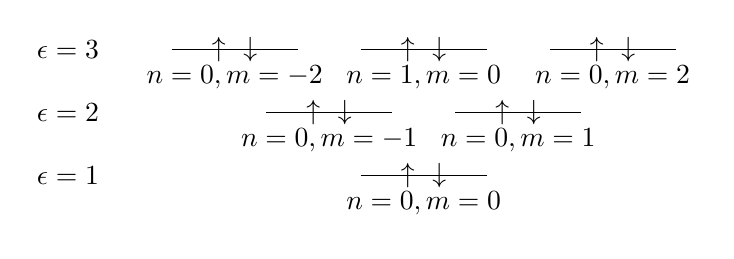
\begin{tikzpicture}[scale=0.8]
                        \begin{scope}
                            \foreach \i in {1, 2, 3} {
                                \draw(-1, \i - 1) node[anchor=east]
                                {$\epsilon = \i$};
                            }

                            % Highest energy level
                            \foreach \i in {0, 3, 6} {
                                \draw (\i, 2) -- (\i + 2, 2);
                                \node at (\i + 0.75, 2) {$\uparrow$};
                                \node at (\i + 1.25, 2) {$\downarrow$};
                            }
                            \node[below, inner sep=.2cm] at (1, 2)
                            {$n = 0, m = -2$};
                            \node[below, inner sep=.2cm] at (4, 2)
                            {$n = 1, m = 0$};
                            \node[below, inner sep=.2cm] at (7, 2)
                            {$n = 0, m = 2$};

                            % Middle energy level
                            \foreach \i in {1.5, 4.5} {
                                \draw (\i, 1) -- (\i + 2, 1);
                                \node at (\i + 0.75, 1) {$\uparrow$};
                                \node at (\i + 1.25, 1) {$\downarrow$};
                            }
                            \node[below, inner sep=.2cm] at (2.5, 1)
                            {$n = 0, m = -1$};
                            \node[below, inner sep=.2cm] at (5.5, 1)
                            {$n = 0, m = 1$};

                            % Lowest energy level
                            \draw (3, 0) -- (5, 0);
                            \node at (3 + 0.75, 0) {$\uparrow$};
                            \node at (3 + 1.25, 0) {$\downarrow$};
                            \node[below, inner sep=.2cm] at (4, 0)
                            {$n = 0, m = 0$};
                        \end{scope}
                    \end{tikzpicture}
                \end{center}
                \caption{In this plot we can see the energy degeneracy of the
                lowest three energy levels in the two-dimensional quantum dot.
                Each arrow representes a spin up or a spin down state with the
                quantum numbers $n$ and $m$ as listed below. This pattern goes
                on indefinitly with the addition of one bar (two oscillators)
                per level.}
                \label{fig:basis_states}
            \end{figure}

            Starting from the bottom and working our way upwards from left to
            right we can label each line from $0$ to $n$ in increasing
            order. This enumeration will serve as our common quantum number
            $\alpha$\footnote{Note that we use greek letters $\alpha, \beta,
            \dots$ for the harmonic oscillator wavefunctions as opposed to latin
            letters for the general indices.}. We will only work with full
            \emph{shells}, i.e., we restrict our views to systems of $N$
            particles where $N$ will be a magic number which we get by counting
            all spin states for each energy level and the energy levels below.
            In \autoref{fig:basis_states} we can see the magic numbers $N \in [2,
            6, 12]$ by counting the levels in increasing order.

            The normalization condition now reads
            \begin{align}
                \braket{\alpha}{\beta}
                = \delta_{\alpha\beta}\delta_{\sigma_\alpha\sigma_\beta},
            \end{align}
            The one-body matrix will be a diagonal matrix with the eigenenergies
            of the single particle harmonic oscillator functions as elements.
            \begin{align}
                \bra{\alpha}h\ket{\beta}
                = \epsilon_{\beta}
                \delta_{\alpha\beta}\delta_{\sigma_\alpha\sigma_\beta}.
            \end{align}

            The two-body matrix elements are a little harder to work out as the
            harmonic oscillator wavefunctions are not eigenfunctions to the
            correlation operator. Luckily, from E. Anisimovas and A.  Matulis
            (Equation A2)\cite{anisimovas1998energy} we can get an analytical
            expression for the two-body matrix elements. We can then construct
            the antisymmetric two-body matrix elements in the harmonic
            oscillator basis.
            \begin{align}
                u^{\alpha\beta}_{\gamma\delta}
                &= \bra{\alpha\beta}u\ket{\gamma\delta}
                - \bra{\alpha\beta}u\ket{\delta\gamma}.
            \end{align}
            Computing the Coulomb elements is an extremely costly operation and
            we will thus only compute the non-zero orbital integrals, i.e., neglecting
            spin and antisymmetry, before saving these to a file which we can
            read several times.

        \subsubsection{Constructing the Hartree-Fock basis}
            Having found the matrix elements of $h$ and $u$ we can now use the
            \emph{self-consistent field} (SCF) iteration method to construct $h$
            and $u$ in a \emph{restricted Hartree-Fock} (RHF) basis. This will
            yield a better estimate to the actual, unknown basis functions of
            the system.

            The neatest, yet arguably the most abstract, way to write the
            Hartree-Fock equations for electron $i$ is
            \begin{equation}
                f \varphi_p = \varepsilon_p \varphi_p,
            \end{equation}
            where $f$ is the Fock operator, $\varphi_p$ are eigenstates of the
            Fock operator consisting of a set of one-electron wave functions
            called the Hartree-Fock molecular orbitals, and $\varepsilon_p$ are
            the eigenenergies of the Fock operator. The Fock operator, in matrix
            notation, is given by
            \begin{equation}
                f^p_q = h^p_q + J(D)^p_q - \half K(D)^p_q,
            \end{equation}
            where $h^p_q$ is the one-body operator, while the two-body operator
            is divided into what we call a direct part,
            \begin{equation}
                J(D)^p_q = \bra{pr}u\ket{qs}D_{sr},
            \end{equation}
            and an exchange part,
            \begin{equation}
                K(D)^p_q = \bra{pr}u\ket{sq}D_{sr}.
            \end{equation}
            Pay special attention to the non-antisymmetric two-body elements in
            the direct and exchange part.  The direct part of the two-body
            operator is comparable to classical Coloumb repulsion, while the
            exchange does not have a classical analog as it arises from the
            antisymmetry requirement of the wavefunction. The matrix $D_{sr}$ is
            the density matrix of the system and will be defined shortly.

            Introducing a basis set transforms the Hartree-Fock equations into
            the Rothaan equations
            \begin{equation}
                FC = SC\varepsilon,
            \end{equation}
            where $F$ is the Fock matrix constructed from $f^p_q$.  This is a
            generalised eigenvalue problem where
            \begin{align}
                S^{p}_{q} = \braket{p}{q},
            \end{align}
            i.e., the \emph{overlap matrix}. We now define the density matrix
            $D$ by
            \begin{align}
                D^{p}_{q} \equiv C^p_{\alpha}{C^{\alpha}_q}^{*},
            \end{align}
            Since the Fock matrix $F$ depends on it's own solution through the
            orbitals, the eigenvalue problem must be solved
            iteratively\footnote{This is also the reason why the Roothan-Hall
            equations are often called the self-consistent-field procedure.}

            Because the RHF SCF method is a variational method, the initial
            wavefunction made up of the single-particle wavefunctions
            $\varphi_i$ is varied until the minimal energy is found.
            \begin{align}
                E_{\text{RHF}}
                &= \para{
                    f^p_q - \half J(D)^p_q + \frac{1}{4}K(D)^p_q
                }D^q_p.
            \end{align}

            The transformations necessary to make all these variations will now
            be contained in $C$. So if we start from a harmonic oscillator (HO)
            basis, $\ket{\alpha}$ we can transform into a better basis, called a
            Hartree-Fock (HF) basis, $\ket{p}$.
            \begin{equation}
                \ket{p}
                = \para{\ket{\alpha}\bra{\alpha}}\ket{p}
                = C^p_\alpha\ket{\alpha}.
            \end{equation}
            We will see how the coupled cluster method with double excitations
            works with both the HO basis and the HF basis, but not equally well.

\section{Implementation}
    We have costructed a flexible framework for performing Hartree-Fock
    self-consistent field iterations and coupled cluster with double excitations
    computations. The entire code base consists of package for
    \lstinline{Python} that is easy to install globally on any computer.

    Because we have employed a mixture of Python and C++ with Cython interfaces,
    the code sturcture may be difficult to understand for someone without Cython
    experience, but we have tried to make the actual usage of the software as
    painless as possible.

    Most of the computations that are done in a coupled cluster algorithm is
    linear algebra and we found that NumPy, relying on BLAS and LAPACK, is quite
    fast and at the very least, efficient enough for our purposes. The quicker
    and easier scripting capabilities Python provides is worth what little extra
    speed-up writing the entire code base in C++ could have provided.

    \subsection{Installation and Usage}

        The software is easy to install by first cloning the GitHub reopsitory,
        \begin{bash}
            git clone git@github.com:Schoyen/FYS4411.git
        \end{bash}
        Then all you need to do is change directory to the project code folder
        where a \lstinline{Makefile} is included so you only need to build and
        install,
        \begin{bash}
            cd FYS4411/project_2/coupled-cluster
            make build
            make install
        \end{bash}
        Now everything should be able to run from anywhere on your computer.  To
        ensure that all requirements of the program are satisfied you can
        install with \mintinline{bash}{make installr} instead. Running
        \mintinline{bash}{py.test} on the command-line in the
        top-directory\footnote{That is, in
        \texttt{FYS4411/project\_2/coupled-cluster}.} will run the test scripts
        located in the \texttt{tests}-directory to make sure that the
        installation passed successfully.

        The script that is used to generate most of the data is located in
        \url{https://github.com/Schoyen/FYS4411/blob/master/project_2/scripts/comparison.py}
        and provides a good example on how to use the code base.

    \subsection{Program Structure}
        There are three main subsetions within our program structure,
        given in the directory tree below.

        \vspace{10pt}
        \dirtree{%
        .1 coupled\_cluster.
            .2 matrix\_elements.
                .3 generate\_matrices.
                .3 index\_map.
            .2 hartree\_fock.
                .3 scf\_rhf.
                .3 basis\_transformation.
            .2 schemes.
                .3 ccd.
                .3 ccd\_sparse.
                .3 ccd\_optimized.
        }
        \vspace{10pt}

        The first subsection, \mintinline{python}{matrix_elemtents},
        contains methods for computing matrix elements in harmonic
        oscillator basis from an analytical
        expression\cite{anisimovas1998energy}.  Computing the matrix
        elements is a very intensive task, and the central functions are
        therefore implemented in C++ with a Cython interface to enable use
        in Python.

        The \mintinline{python}{hartree_fock} subsection contains methods
        for changing from harmonic oscillator basis to Hartree-Fock basis as
        well as an implementation of the self-consistent-field algorithm to
        make this transaction possible.

        The \mintinline{python}{schemes} subsection is arguably the most
        important part of this project. The subsection has three different
        classes that perform the exact same computations, but in different
        and increasingly intelligent ways. First,
        \mintinline{python}{CoupledClusterDoubles} is the most
        straightforward and naïve way to solve the CCD amplitude equations.
        Second, because an overbearing amount of the elements in the
        operator matrices in this problem are zero, we have implemented a
        sparse matrix CDD solver in
        \mintinline{python}{CoupledClusterDoublesSparse}. Third,
        \mintinline{python}{CoupledClusterDoublesOptimized} takes advantage
        of sparse matrices as well, but is also parallellized and optimized
        with memory use and number of floating point operations in mind.

        Both in \mintinline{python}{CoupledClusterDoublesSparse} and
        \mintinline{python}{CoupledClusterDoublesOptimized} we make use
        of the intermediates in equations \ref{eq:intermediate1} to
        \ref{eq:intermediate4}. We have also relied upon implementations
        in C++ for some of the heaviest computations. In the optimized
        class special care was taken to ensure that every contraction
        was computed in an optimal way, with the minimization of memory
        use and CPU time as the overall goal. Moreover, several methods
        in NumPy for doing linear algebra was tested, including but not limited
        to \mintinline{python}{numpy.einsum()}, \mintinline{python}{numpy.tensordot},
        and reshaping datastructures to two dimensions and using
        \mintinline{python}{numpy.dot}. Additionally, we tried to make use of
        the python package \mintinline{python}{dask} which allows for arrays that
        are larger than the computer's memory buffer as well as automated
        concurrency. We found that the dask arrays was a bad fit for our code
        base, but we ended up using \mintinline{python}{numba} for automated
        paralellization of some iterative loops as well as just-in-time
        compialtion of some functions.

    \subsection{Scaling of the coupled cluster doubles method}
        \label{subsec:ccd_scaling}

    \subsection{Convergence Problems and Mixing}

        Iterative many-body methods are prone to convergence problems for some
        configurations. Since Hartree-Fock is a variational method, SCF convergence
        is found when the energy is stationary with respect to inifitesimal
        variations in the orbitals. Unfortunately, the SCF iteration scheme does
        not always converge. Luckily, numerous techniques exist for controlling
        and accelerating convergence\cite{schlegel1991you}. The same kind of
        methods have proven useful to ensure convergence of coupled cluster methods
        \cite{scuseria1986accelerating}.

        The simplest way to try to ``massage'' convergence out of the CCD-method
        is to use \emph{damping} where you include a part of the result from the
        previous iteration i.e.,
        \begin{align}
            \tilde{t}^{k + 1} = \theta t^{k + 1} + (1 - \theta)t^k,
            \label{eq:mixing}
        \end{align}
        where $t^{k + 1}$ is the current value computed using
        \autoref{eq:iterative_amplitude} and $t^k$ is the previous value for the
        amplitude. Choosing $\theta \in [0, 1]$ we can tune how much of the
        previous amplitude we wish to include in the new state. This allows for
        a more gradual transition between the iterations. We now use
        $\tilde{t}^{k + 1}$ as our estimate of the new amplitude.

        A more sophisticated mixing method is the direct inversion
        in the iterative subspace (DIIS), also known as Pulay mixing. While the
        common mixing method is used for many other applications
        \footnote{It is, for instance, called an alpha filter in data acquisition.},
        the DIIS method is developed with the sole intent of accelerating
        convergense in Hartree-Fock methods. In DIIS one would construct a
        linear combinations of approximate errors from previous iterations,
        analogous to a very clever weighted moving average. We have not implemented
        this scheme, but it nevertheless warrants mention.

\section{Results}

    \subsection{Ground state energies for two-dimensional quantum dots}
        Here we show the ground state energies for the two-dimensional quantum
        dots using restriced Hartree-Fock (RHF), coupled cluster doubles using
        both the harmonic oscillator basis and the Hartree-Fock basis which we
        construct after running the RHF-method. We have chosen the convergence
        criteria to be $\num{1e-6}$ in our results for the sake of comparison
        with M. P. Lohne\cite{lohne2011ab}.

        All the results from our simulations are displayed in tables \ref{tab:N2},
        \ref{tab:N6}, \ref{tab:N12} and \ref{tab:N20}. They show the ground state
        energy as a result of restricted Hartree-Fock SCF iterations, and coupled
        cluster doubles with harmonic oscillator basis and Hatree-Fock basis for
        systems of increasing size, $N=2$, $N=6$, $N=12$ and $N=20$ particles
        respectively. The results are thoroughtly discussed in the next section.

        \begin{table}
            \centering
            \caption{Results for $N = 2$ particles, where convergence was
            achieved for all parameters. Taut's\cite{taut1994two} analytic
            result for $\omega = 1.0$ a.u. is $3$.}
            \begin{ruledtabular}
                \begin{tabular}{c|c|ccc}
                    $\omega$ & $R$ & RHF & CCD(HO) & CCD(HF) \\
                    \hline
                               &  $1$  & $0.596333$ & $0.596333$ & $0.596333$ \\
                               &  $2$  & $0.596333$ & $0.512520$ & $0.512520$ \\
                               &  $3$  & $0.526903$ & $0.505972$ & $0.442235$ \\
                               &  $4$  & $0.526903$ & $0.499216$ & $0.442011$ \\
                               &  $5$  & $0.525666$ & $0.497172$ & $0.443293$ \\
        \multirow{2}{*}{$0.1$} &  $6$  & $0.525666$ & $0.494232$ & $0.443145$ \\
                               &  $7$  & $0.525635$ & $0.493142$ & $0.443056$ \\
                               &  $8$  & $0.525635$ & $0.491895$ & $0.442981$ \\
                               &  $9$  & $0.525635$ & $0.491262$ & $0.442927$ \\
                               &  $10$ & $0.525635$ & $0.490649$ & $0.442886$ \\
                               &  $11$ & $0.525635$ & $0.490262$ & $0.442853$ \\
                               &  $12$ & $0.525635$ & $0.489918$ & $0.442827$ \\
                    \hline

                               &  $1$  & $1.886227$ & $1.886227$ & $1.886227$ \\
                               &  $2$  & $1.886227$ & $1.786914$ & $1.786914$ \\
                               &  $3$  & $1.799856$ & $1.778903$ & $1.681979$ \\
                               &  $4$  & $1.799856$ & $1.760117$ & $1.673881$ \\
                               &  $5$  & $1.799748$ & $1.754385$ & $1.670053$ \\
        \multirow{2}{*}{$0.5$} &  $6$  & $1.799748$ & $1.748232$ & $1.667804$ \\
                               &  $7$  & $1.799745$ & $1.745231$ & $1.666474$ \\
                               &  $8$  & $1.799745$ & $1.742548$ & $1.665494$ \\
                               &  $9$  & $1.799743$ & $1.740860$ & $1.664805$ \\
                               &  $10$ & $1.799743$ & $1.739444$ & $1.664270$ \\
                               &  $11$ & $1.799742$ & $1.738416$ & $1.663856$ \\
                               &  $12$ & $1.799742$ & $1.737562$ & $1.663522$ \\
                    \hline

                               &  $1$  & $3.253314$ & $3.253314$ & $3.253314$ \\
                               &  $2$  & $3.253314$ & $3.152328$ & $3.152328$ \\
                               &  $3$  & $3.162691$ & $3.141827$ & $3.039048$ \\
                               &  $4$  & $3.162691$ & $3.118679$ & $3.025273$ \\
                               &  $5$  & $3.161921$ & $3.110967$ & $3.017944$ \\
        \multirow{2}{*}{$1.0$} &  $6$  & $3.161921$ & $3.103338$ & $3.013923$ \\
                               &  $7$  & $3.161909$ & $3.099324$ & $3.011405$ \\
                               &  $8$  & $3.161909$ & $3.095916$ & $3.009621$ \\
                               &  $9$  & $3.161909$ & $3.093662$ & $3.008343$ \\
                               &  $10$ & $3.161909$ & $3.091818$ & $3.007357$ \\
                               &  $11$ & $3.161909$ & $3.090436$ & $3.006590$ \\
                               &  $12$ & $3.161909$ & $3.089299$ & $3.005970$ \\
                    \hline

                               &  $1$  & $5.772454$ & $5.772454$ & $5.772454$ \\
                               &  $2$  & $5.772454$ & $5.671234$ & $5.671234$ \\
                               &  $3$  & $5.679048$ & $5.658272$ & $5.553528$ \\
                               &  $4$  & $5.679048$ & $5.631669$ & $5.534333$ \\
                               &  $5$  & $5.677282$ & $5.622092$ & $5.523490$ \\
        \multirow{2}{*}{$2.0$} &  $6$  & $5.677282$ & $5.613118$ & $5.517552$ \\
                               &  $7$  & $5.677206$ & $5.608130$ & $5.513709$ \\
                               &  $8$  & $5.677206$ & $5.604026$ & $5.511012$ \\
                               &  $9$  & $5.677204$ & $5.601216$ & $5.509050$ \\
                               &  $10$ & $5.677204$ & $5.598946$ & $5.507540$ \\
                               &  $11$ & $5.677204$ & $5.597213$ & $5.506356$ \\
                               &  $12$ & $5.677204$ & $5.595791$ & $5.505399$
                \end{tabular}
            \end{ruledtabular}
            \label{tab:N2}
        \end{table}

        \begin{table}
            \centering
            \caption{Results for $N = 6$ particles. No convergence is marked as
            {\nan} in the table. For low frequencies the CCD-method using the HO
            basis has a hard time achieving convergence.}
            \begin{ruledtabular}
                \begin{tabular}{c|c|ccc}
                    $\omega$ & $R$ & RHF & CCD(HO) & CCD(HF) \\ \hline
                             &  $2$  & $4.864244$ & $4.864244$ & $4.864244$ \\
                             &  $3$  & $4.435740$ & $4.446235$ & $4.319901$ \\
                             &  $4$  & $4.019787$ & $4.383692$ & $3.829962$ \\
                             &  $5$  & $3.963149$ & \nan & $3.666722$ \\
                             &  $6$  & $3.870617$ & \nan & $3.597876$ \\
                      $0.1$  &  $7$  & $3.863135$ & \nan & $3.590388$ \\
                             &  $8$  & $3.852880$ & \nan & $3.587711$ \\
                             &  $9$  & $3.852591$ & \nan & $3.587291$ \\
                             &  $10$ & $3.852393$ & \nan & $3.587136$ \\
                             &  $11$ & $3.852391$ & \nan & $3.586821$ \\
                             &  $12$ & $3.852382$ & \nan & $3.586582$ \\ \hline

                             &  $2$  & $13.640713$ & $13.640713$ & $13.640713$ \\
                             &  $3$  & $13.051620$ & $13.385987$ & $12.901520$ \\
                             &  $4$  & $12.357471$ & $13.261097$ & $12.057345$ \\
                             &  $5$  & $12.325128$ & $13.138572$ & $11.934988$ \\
                             &  $6$  & $12.271499$ & $13.084158$ & $11.864098$ \\
                      $0.5$  &  $7$  & $12.271375$ & $13.068399$ & $11.849762$ \\
                             &  $8$  & $12.271361$ & $13.055561$ & $11.841330$ \\
                             &  $9$  & $12.271337$ & $13.045386$ & $11.835470$ \\
                             &  $10$ & $12.271326$ & $13.037878$ & $11.831351$ \\
                             &  $11$ & $12.271324$ & \nan & $11.828242$ \\
                             &  $12$ & $12.271320$ & \nan & $11.825835$ \\ \hline

                             &  $2$  & $22.219813$ & $22.219813$ & $22.219813$ \\
                             &  $3$  & $21.593198$ & $21.974675$ & $21.423811$ \\
                             &  $4$  & $20.766919$ & $21.854191$ & $20.429265$ \\
                             &  $5$  & $20.748402$ & $21.793624$ & $20.332454$ \\
                             &  $6$  & $20.720257$ & $21.750091$ & $20.274013$ \\
                      $1.0$  &  $7$  & $20.720132$ & $21.718843$ & $20.249849$ \\
                             &  $8$  & $20.719248$ & $21.695224$ & $20.234705$ \\
                             &  $9$  & $20.719248$ & $21.675931$ & $20.224389$ \\
                             &  $10$ & $20.719217$ & $21.661830$ & $20.217075$ \\
                             &  $11$ & $20.719215$ & $21.649812$ & $20.211541$ \\
                             &  $12$ & $20.719215$ & $21.640765$ & $20.207258$ \\
                             \hline

                             &  $2$  & $37.281425$ & $37.281425$ & $37.281425$ \\
                             &  $3$  & $36.637217$ & $37.042127$ & $36.450634$ \\
                             &  $4$  & $35.689555$ & $36.925664$ & $35.328432$ \\
                             &  $5$  & $35.681729$ & $36.864367$ & $35.250185$ \\
                             &  $6$  & $35.672333$ & $36.812895$ & $35.200308$ \\
                      $2.0$  &  $7$  & $35.671851$ & $36.775986$ & $35.168245$ \\
                             &  $8$  & $35.670358$ & $36.747864$ & $35.147097$ \\
                             &  $9$  & $35.670333$ & $36.725261$ & $35.131953$ \\
                             &  $10$ & $35.670144$ & $36.708362$ & $35.121033$ \\
                             &  $11$ & $35.670143$ & $36.694188$ & $35.112680$ \\
                             &  $12$ & $35.670127$ & $36.683281$ & $35.106188$
                \end{tabular}
            \end{ruledtabular}
            \label{tab:N6}
        \end{table}

        \begin{table}
            \centering
            \caption{Here we look at $N = 12$ particles ($R = 3$ shells).  We did
            not achieve convergence using the harmonic oscillator basis for the
            lower frequency values and large number of shells. No convergence is
            marked as {\nan} in the table.}
            \begin{ruledtabular}
                \begin{tabular}{c|c|ccc}
                    $\omega$ & $R$ & RHF & CCD(HO) & CCD(HF) \\
                    \hline
                          & $3$ & $46.361130$ & $46.361130$ & $46.361130$ \\
                          & $4$ & $43.663267$ & $45.837079$ & $43.309845$ \\
                          & $5$ & $41.108851$ & $45.456883$ & $40.654710$ \\
                          & $6$ & $40.750512$ & \nan & $40.068340$ \\
                    $0.5$ & $7$ & $40.302719$ & \nan & $39.508500$ \\
                          & $8$ & $40.263752$ & \nan & $39.399128$ \\
                          & $9$ & $40.216688$ & \nan & $39.329311$ \\
                          & $10$ & $40.216252$ & \nan & $39.309409$ \\
                          & $11$ & $40.216195$ & \nan & $39.296007$ \\
                          & $12$ & $40.216165$ & \nan & $39.285968$ \\
                    \hline
                          & $3$ & $73.765549$ & $73.765549$ & $73.765549$ \\
                          & $4$ & $70.673849$ & $73.314476$ & $70.324250$ \\
                          & $5$ & $67.569930$ & $72.990679$ & $67.031096$ \\
                          & $6$ & $67.296869$ & \nan & $66.526677$ \\
                    $1.0$ & $7$ & $66.934745$ & \nan & $66.049564$ \\
                          & $8$ & $66.923094$ & \nan & $65.972157$ \\
                          & $9$ & $66.912244$ & \nan & $65.921205$ \\
                          & $10$ & $66.912035$ & \nan & $65.889281$ \\
                          & $11$ & $66.911365$ & \nan & $65.866715$ \\
                          & $12$ & $66.911364$ & \nan & $65.849776$ \\
                    \hline
                          & $3$ & $120.722260$ & $120.722260$ & $120.722260$ \\
                          & $4$ & $117.339642$ & $120.296556$ & $116.995036$ \\
                          & $5$ & $113.660396$ & $120.007146$ & $113.048934$ \\
                          & $6$ & $113.484866$ & $119.759037$ & $112.658821$ \\
                    $2.0$ & $7$ & $113.247601$ & $119.662199$ & $112.309482$ \\
                          & $8$ & $113.246579$ & $119.584733$ & $112.235521$ \\
                          & $9$ & $113.246303$ & $119.524394$ & $112.181828$ \\
                          & $10$ & $113.245854$ & $119.472283$ & $112.140661$ \\
                          & $11$ & $113.245256$ & $119.430353$ & $112.109973$ \\
                          & $12$ & $113.245183$ & $119.394712$ & $112.085683$ \\
                    \hline
                          & $3$ & $242.334879$ & $242.334879$ & $242.334879$ \\
                          & $4$ & $238.739591$ & $241.927593$ & $238.394598$ \\
                          & $5$ & $234.352741$ & $241.663950$ & $233.680649$ \\
                          & $6$ & $234.282331$ & $241.507595$ & $233.425243$ \\
                    $5.0$ & $7$ & $234.194820$ & $241.390525$ & $233.226529$ \\
                          & $8$ & $234.194059$ & $241.293417$ & $233.137933$ \\
                          & $9$ & $234.190797$ & $241.221056$ & $233.070205$ \\
                          & $10$ & $234.190714$ & $241.158896$ & $233.020009$ \\
                          & $11$ & $234.190665$ & $241.109926$ & $232.980634$ \\
                          & $12$ & $234.190553$ & $241.068091$ & $232.948528$
                \end{tabular}
            \end{ruledtabular}
            \label{tab:N12}
        \end{table}

        \begin{table}
            \centering
            \caption{In this table we look at $N = 20$ particles ($R = 4$
            shells).  We did not achieve convergence using the harmonic
            oscillator basis for the lower frequency values and large number of
            shells. No convergence is marked as {\nan} in the table.}
            \begin{ruledtabular}
                \begin{tabular}{c|c|ccc}
                    $\omega$ & $R$ & RHF & CCD(HO) & CCD(HF) \\
                    \hline
                          & $4$ & $177.963297$ & $177.963297$ & $177.963297$ \\
                          & $5$ & $168.792442$ & $177.206536$ & $168.459124$ \\
                          & $6$ & $161.339721$ & \nan & $160.594507$ \\
                          & $7$ & $159.958722$ & \nan & $158.841120$ \\
                    $1.0$ & $8$ & $158.400172$ & \nan & $157.038330$ \\
                          & $9$ & $158.226030$ & \nan & $156.676039$ \\
                          & $10$ & $158.017667$ & \nan & $156.367930$ \\
                          & $11$ & $158.010276$ & \nan & $156.292422$ \\
                          & $12$ & $158.004951$ & \nan & $156.238258$ \\
                    \hline
                          & $4$ & $286.825295$ & $286.825295$ & $286.825295$ \\
                          & $5$ & $276.898196$ & $286.159148$ & $276.381708$ \\
                          & $6$ & $267.269712$ & $285.614958$ & $266.413122$ \\
                          & $7$ & $266.213200$ & \nan & $264.969415$ \\
                    $2.0$ & $8$ & $264.933622$ & \nan & $263.434546$ \\
                          & $9$ & $264.874009$ & \nan & $263.215451$ \\
                          & $10$ & $264.809954$ & \nan & $263.046195$ \\
                          & $11$ & $264.809901$ & \nan & $262.963703$ \\
                          & $12$ & $264.809306$ & \nan & $262.899698$ \\
                    \hline
                          & $4$ & $563.773952$ & $563.773952$ & $563.773952$ \\
                          & $5$ & $552.630093$ & $563.160136$ & $552.118708$ \\
                          & $6$ & $540.804720$ & $562.692231$ & $539.824400$ \\
                          & $7$ & $540.227793$ & $562.306123$ & $538.886074$ \\
                    $5.0$ & $8$ & $539.499326$ & $562.114279$ & $537.925127$ \\
                          & $9$ & $539.495941$ & \nan & $537.769045$ \\
                          & $10$ & $539.494611$ & \nan & $537.646668$ \\
                          & $11$ & $539.493513$ & \nan & $537.548828$ \\
                          & $12$ & $539.491764$ & \nan & $537.470616$ \\
                    \hline
                           & $4$ & $973.032700$ & $973.032700$ & $973.032700$ \\
                           & $5$ & $961.371081$ & $972.439478$ & $960.862053$ \\
                           & $6$ & $948.057077$ & $972.002302$ & $947.019789$ \\
                           & $7$ & $947.765474$ & $971.716015$ & $946.399546$ \\
                    $10.0$ & $8$ & $947.410305$ & $971.508584$ & $945.827806$ \\
                           & $9$ & $947.409440$ & $971.332133$ & $945.663820$ \\
                           & $10$ & $947.404930$ & $971.193592$ & $945.528489$ \\
                           & $11$ & $947.404361$ & $971.076617$ & $945.424175$ \\
                           & $12$ & $947.403875$ & $970.978571$ & $945.339080$ \\
                \end{tabular}
            \end{ruledtabular}
            \label{tab:N20}
        \end{table}

    \subsection{Running time}
        Here we show how the three implementations of the CCD-method scales as a
        function of the shell number $R$ for $N = 2$ and $N = 6$, in table
        \ref{fig:running_time_2} and \ref{fig:running_time_6} respectively. The same
        behaviour is shown for higher number of particles. In \autoref{fig:running_time_6_zoom}
        we have plotted the computation time for $N=6$ particles again, but we
        have excluded the naïve method for better comparison of the sparse and
        optimized method.

        \begin{figure}
            \centering
            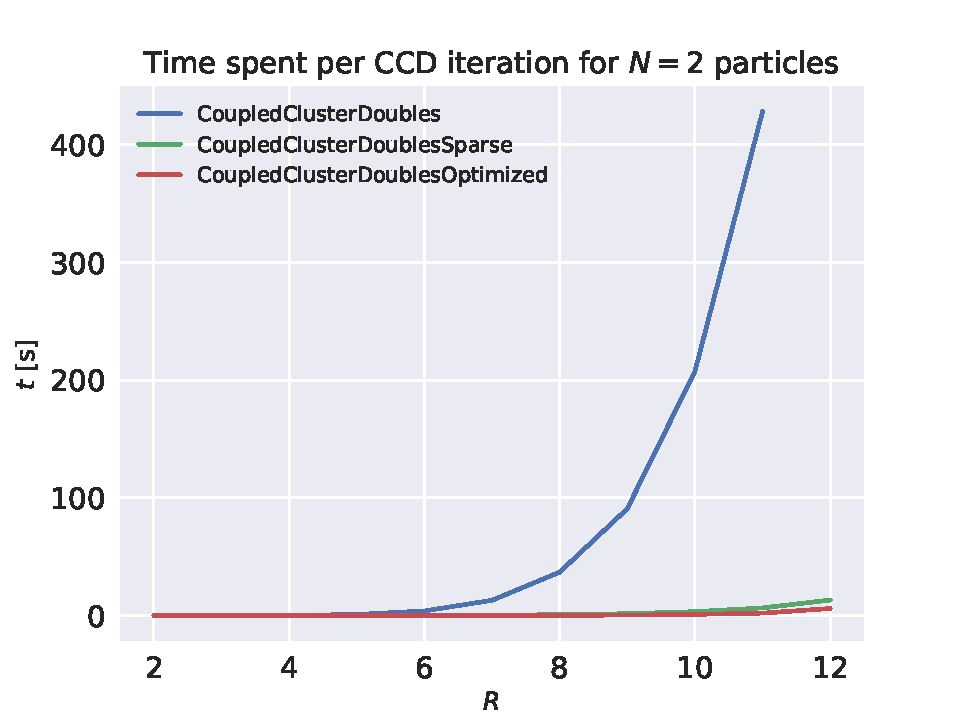
\includegraphics[width=244px]
            {../dat/figures/iter_run_times_2.pdf}
            \caption{In this figure we can see the running time per iteration
            for $N = 2$ particles as a function of the shell number $R$. We did
            not run the naïve implementation for $R = 12$.}
            \label{fig:running_time_2}
        \end{figure}

        \begin{figure}
            \centering
            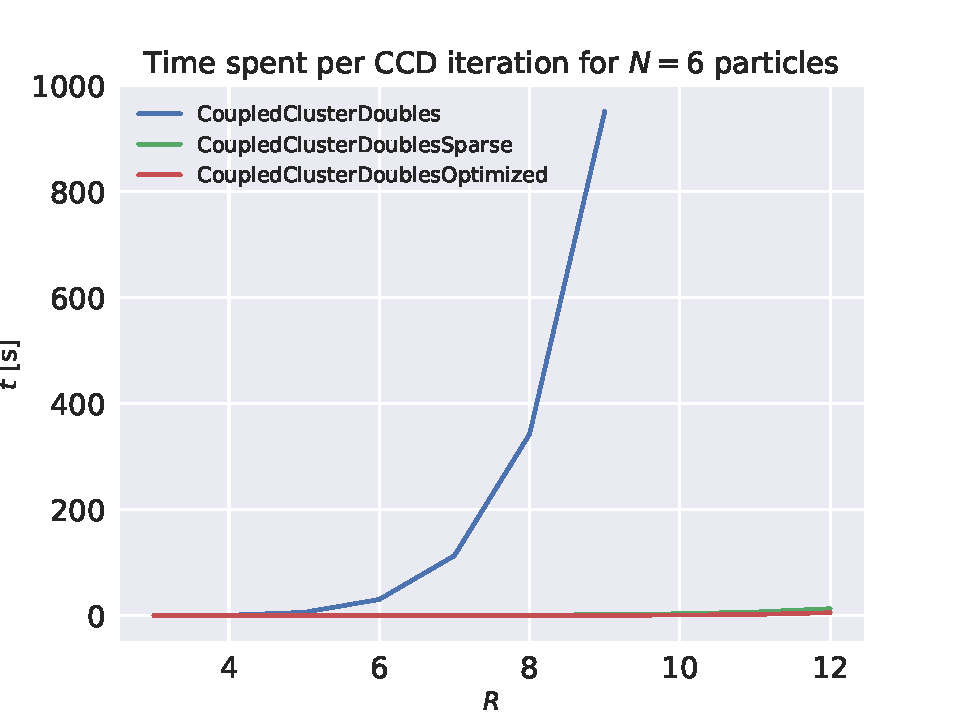
\includegraphics[width=244px]
            {../dat/figures/iter_run_times_6.pdf}
            \caption{Here we see the running time per iteration for $N = 6$
            particles as a function of the shell number $R$. We did not run the
            naïve implementation for $R > 9$ in this figure.}
            \label{fig:running_time_6}
        \end{figure}

        \begin{figure}
           \centering
            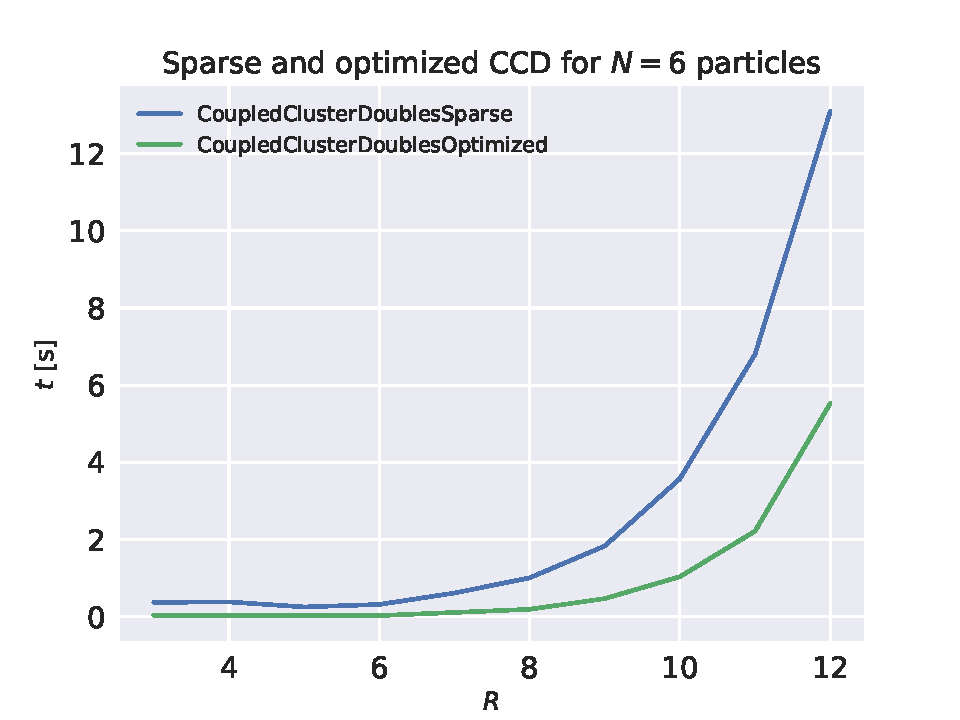
\includegraphics[width=244px]
            {../dat/figures/iter_run_times_zoom_6.pdf}
            \caption{Run time for $N=6$ particles, only the faster methods are
            included for better comparison.}
            \label{fig:running_time_6_zoom}
        \end{figure}

\section{Discussion}

    \subsection{Performance comparison}
        Somewhat surprisingly, the Hartree-Fock method outperforms the coupled
        cluster doubles when the harmonic oscillator basis is used. This
        happens for almost any configuration except the smallest system
        with $N=2$ particles. This comes from the fact that the HO basis is
        not very good at representing the states in the system. As we have
        already stated, because the Hartree-Fock SCF iterations is a variational
        methdod, the basis is varied in order to find the minimal energy. The new
        basis states will be linear combinations of the old basis states. When
        the iterations are finished, the new transformed HF basis will then be
        much better at representing the possible quantum configurations compared
        to the HO basis. This effect is only apparent in system with a larger
        number of particles and/or low frequency. This is because in a system with
        a large number of particles relative to the frequency particle-particle
        interaction will be more prominent than the harmonic oscillator potential
        the particles are subject to. I other words, the HO basis would fit rather
        well.

    \subsection{Validity of results}
        The analytical computed energy for $\omega=1.0$ a.u.
        and $N=2$ is $3$\cite{taut1994two}. From our tables we see
        that RHF is least successful in reaching this value, CCD in
        HF basis is best, while CCD with HO basis is generally somewhere
        between the two. We see that we get even closer to the analytical
        ``truth'' by increasing the number of shells.

        The rest of results have been compared with the master thesis of M. P.
        Lohne\cite{lohne2010coupled} for up to 10 shells. Lohne gets two sets of
        energies, one set from RHF and one set from CCSD code with harmonic
        oscillator basis functions. Our CCD code with Hartree-Fock basis will
        for some configurations\footnote{By configurations we mean frequency
        $\omega$ and number of particles $N$.} beat CCSD with plain harmonic
        oscillator basis. For 12 shells we can compare with the results from M.
        P. Lohne et al.\cite{lohne2011ab}, but in this article an
        \emph{effective interaction} for the Hamiltonian with a CCSD code has
        been used. These results are therefore significanlty better than ours,
        but we can get a ``ball-park'' idea to benchmark against.

    \subsection{Running time}
        Looking at the running times shown in \autoref{fig:running_time_2} and
        \autoref{fig:running_time_6} we can see how the naïve implementation
        blows up very fast. As both the sparse and the optimized version uses
        intermediate calculations these running times scales on the order of
        $\mathcal{O}(l^6)$ whereas the naïve implementation goes as
        $\mathcal{O}(l^8)$. Another important factor is that the naïve
        implementation uses \texttt{np.einsum} to calculate the tensor
        contractions whereas the sparse and optimized version uses
        \texttt{sparse.tensordot} and \texttt{np.matmul} respectively. The two
        latter function calls uses BLAS's implementation of the matrix dot which
        is way faster than Numpys \texttt{np.einsum}.

    \subsection{Convergence trouble}
        For a large number of particles and a low frequency the CCD-method get
        trouble with convergence. This happens as the confining potential $v
        \propto \omega^2$ will not be able to confine the particles when the
        interaction gets too strong. The CCD-method will in particular get a
        hard time keep the particles together as the excitation operator $t$
        only excites pairs of particles leading to a too strong increase in the
        interaction when the particles increase their energy level. This effect
        can potentially be somewhat alleviated by including the singles
        excitation, e.g., using the CCSD-method.

        We can see this behaviour in our results. For $N = 2$ we get convergence
        for all methods for $\omega = 0.1$ shown in \autoref{tab:N2}. By
        increasing to $N = 6$ particles we immediately see how CCD with the HO
        basis will get in trouble for small values of $\omega$. Even by increasing
        the strength of the confinment this method does converge.

        For $N = 6$ none of the methods converged when $\omega =
        0.1$\footnote{The RHF-method would probably have converged if we had
        started tuning its mixing parameter, but as we have focused on CCD we did
        not think it relevant to include these results.}. By increasing the
        frequency we restored the convergence. For larger number of shells we
        had to start increasing the value of $\theta \to 0.9$ in order to get
        convergence within the threshold.

        CCD with HO basis experiences the same convergence problems also for,
        $N=12$ particles and for $N=20$ particles.

    %\subsection{Sparse implementation}
    % Did you want to write something about memory use, Oyvind? Memory problems?

    \section{Summary Remarks}

        Our main product from this is a product that can do both computations with
        restricted Hartree-Fock (RHF) self-consistent field and coupled cluster
        doubles (CCD). We have tried
        to make a package in python that should be easy enough for anyone to test.
        Moreover we hav demonstrated that one can speed up the computation time with
        a relatively simple algebraic transformation and finding the ``intermediates''.
        The computational speed was further reduced using sparse matrices. It should
        be noted, as a warning, that there are relatively few systems adequately sparese
        for this to work. We added upon the program to increase it further with
        paralellization and optimal use of numerical functions.

        In order to perform the computations we have constructed a harmonic oscillator
        basis. We saw how the CCD method was outperformed RHF in most cases, and often
        exhibited convergence problems. The remedy for these shortcomings is to use
        the Hartree-Fock basis which is provided after successful convergence of
        SCF iterations. The results are improved markedly and classification of coupled
        cluster methods as a post-Harte-Fock method is justified.

        The coupled cluster method provides surprisingly good results even
        though one only includes double esctiations. The reason for this is that
        particle-particle interactions is the amongt the most important thing that
        happens in a ferminon system, second only to no interaction at all, i.e
        what particles do on their own. The way to improve the computations is to
        include other types of excitations like singles (CCSD) and triples (CCSDT),
        add more basis functions, and/or supplement the coupled cluster method with
        another method like a perturbative one. All of this will, needless to say,
        increase the compute time, which must be balanced against the accuracy needed
        for the situation at hand.

\vfill
\newpage
\appendix
\section{The normal ordered Hamiltonian}
    When constructing the normal ordered Hamiltonian we use Wick's theorem to
    write the one-body, $h$, and the two-body, $u$, operators onto a normal
    ordered form. Specifically we define the normal ordered form in terms of the
    \emph{Fermi vacuum}\footnote{Fermi vacuum defines the reference state, i.e.,
    $\kslat$, as the vacuum.}. That is, an operator on normal ordered form
    destroys the reference Slater determinant.

    We start by writing the one-body operator, $h$, to its normal-ordered form.
    \begin{align}
        h &= \sum_{pq}h^p_q\acr{p}\ade{q}
        = \sum_{pq}h^p_q\para{
            \{\acr{p}\ade{q}\}
            + \{
                \wick{\c a_{p}^{\dagger} \c a_{q}}
            \}
        }
        \\
        &= \sum_{pq}h^p_q\{
            \acr{p}\ade{q}
        \}
        + \sum_{pq}h^p_q\delta_{p \in i}\delta_{pq}
        \\
        &= h_N + \sum_{i}h^i_i,
    \end{align}
    where we have used $\delta_{p \in i}$ to mean that $p$ must be an occupied
    index. Doing the same for the two-body operator is a slightly more tedious
    endeavor. For brevity we will only write out the operator strings and only
    keep the non-zero contributions.
    \begin{align}
        \acr{p}\acr{q}\ade{s}\ade{r}
        &=
        \{\acr{p}\acr{q}\ade{s}\ade{r}\}
        + \{
            \wick{\c a_p^{\dagger} a_{q}^{\dagger} \c a_{s} a_{r}}
        \}
        + \{
            \wick{\c a_p^{\dagger} a_{q}^{\dagger} a_{s} \c a_{r}}
        \}
        \nonumber \\
        &\qquad
        + \{
            \wick{a_p^{\dagger} \c a_{q}^{\dagger} \c a_{s} a_{r}}
        \}
        + \{
            \wick{a_p^{\dagger} \c a_{q}^{\dagger} a_{s} \c a_{r}}
        \}
        \nonumber \\
        &\qquad
        + \{
            \wick{\c1 a_p^{\dagger} \c2 a_{q}^{\dagger} \c1 a_{s} \c2 a_{r}}
        \}
        + \{
            \wick{\c2 a_p^{\dagger} \c1 a_{q}^{\dagger} \c1 a_{s} \c2 a_{r}}
        \}
        \\
        &=
        \{\acr{p}\acr{q}\ade{s}\ade{r}\}
        - \delta_{p \in i}\delta_{ps}\{\acr{q}\ade{r}\}
        + \delta_{p \in i}\delta_{pr}\{\acr{q}\ade{s}\}
        \nonumber \\
        &\qquad
        + \delta_{q \in i}\delta_{qs}\{\acr{p}\ade{r}\}
        - \delta_{q \in i}\delta_{qr}\{\acr{p}\ade{s}\}
        \nonumber \\
        &\qquad
        - \delta_{p \in i}\delta_{ps}\delta_{q \in j}\delta_{qr}
        + \delta_{p \in i}\delta_{pr}\delta_{q \in j}\delta_{qs}.
    \end{align}
    Inserted into the full two-body operator and sorting out the sums we get
    \begin{align}
        u
        &=
        \frac{1}{4}\sum_{pqrs}\bra{pq}\ket{rs}
        \{\acr{p}\acr{q}\ade{s}\ade{r}\}
        - \frac{1}{4}\sum_{iqr}\bra{iq}\ket{ri}\{\acr{q}\ade{r}\}
        \nonumber \\
        &\qquad
        + \frac{1}{4}\sum_{iqs}\bra{iq}\ket{is}\{\acr{q}\ade{s}\}
        + \frac{1}{4}\sum_{pir}\bra{pi}\ket{ri}\{\acr{p}\ade{r}\}
        \nonumber \\
        &\qquad
        - \frac{1}{4}\sum_{pis}\bra{pi}\ket{is}\{\acr{p}\ade{s}\}
        - \frac{1}{4}\sum_{ij}\bra{ij}\ket{ji}
        \nonumber \\
        &\qquad
        + \frac{1}{4}\sum_{ij}\bra{ij}\ket{ij}.
    \end{align}
    Using the antisymmetric properties of the two-body matrix elements,
    \begin{align}
        \bra{pq}\ket{rs}
        = - \bra{pq}\ket{sr}
        = - \bra{qp}\ket{rs}
        = \bra{qp}\ket{sr},
    \end{align}
    and relabeling of the indices we can rearrange and collect some terms.
    \begin{align}
        u
        &=
        W_N + \sum_{pir}\bra{pi}\ket{ri}\{\acr{p}\ade{r}\}
        + \half\sum_{ij}\bra{ij}\ket{ij},
    \end{align}
    where the normal ordered two-body operator is
    \begin{align}
        W_N = \frac{1}{4}\sum_{pqrs}
        \bra{pq}\ket{rs}\{\acr{p}\acr{q}\ade{s}\ade{r}\}.
    \end{align}
    When we now construct the full Hamiltonian we can collect some terms. The
    constants in both the one-body and the two-body operator in total constitues
    the reference energy.
    \begin{align}
        E_0 \equiv \bslat H\kslat
        = \sum_{i}h_i^i + \frac{1}{2}\sum_{ij}\bra{ij}\ket{ij}.
        \label{eq:reference_energy}
    \end{align}
    Combining the normal ordered one-body operator and the second term in the
    two-body operator, i.e., the term with a single creation and annihilation
    operator pair, we get the normal ordered Fock-operator.
    \begin{align}
        F_N
        &=
        \sum_{pq}h_{q}^{p}\{\acr{p}\ade{q}\}
        + \sum_{pqi}\bra{pi}\ket{qi}\{\acr{p}\ade{q}\}
        \\
        &= \sum_{pq}f_{q}^{p}\{\acr{p}\ade{q}\},
    \end{align}
    where we have defined the Fock matrix elements as
    \begin{align}
        f_{q}^{p}
        &=
        h_q^p + \sum_{i}\bra{pi}\ket{qi}.
    \end{align}
    In total we get the full Hamiltonian
    \begin{align}
        H
        &=
        F_N + W_N + \bslat H\kslat
        \\
        &= H_N + \bslat H\kslat,
    \end{align}
    which is what we wanted to show.\cite{crawford2007introduction}

\section{Energy equation}
    \label{app:energy_equation}
    Here we show how to compute the coupled cluster doubles energy from
    \autoref{eq:ccd_energy}. The first two terms come from the reference energy
    shown in \autoref{eq:reference_energy}. The last term we get by using Wick's
    theorem.
    \begin{align}
        \bslat (H_N T_2)_c\kslat
        &= \bslat (W_N T_2)_c\kslat,
    \end{align}
    as the normal ordered Fock operator can at most relax a single state, i.e.,
    \begin{align}
        \bslat (F_N T_2)_c\kslat = 0.
    \end{align}
    We are thus left with computing the contraction of the doubles cluster
    operator and the normal ordered two-body operator. Note that we must keep
    only the fully contracted terms.
    \begin{align}
        \bslat (W_N T_2)_c\kslat
        &=
        \frac{1}{16} u^{pq}_{rs} t^{ab}_{ij}
        \bslat
        A
        \kslat,
        \label{eq:third_term_ccd_energy}
    \end{align}
    where $A$ is the create and destruction operator strings. By using
    generalized Wick's theorem we get
    \begin{align}
        A &=
        \{\acr{p}\acr{q}\ade{s}\ade{r}\}
        \{\acr{a}\acr{b}\ade{j}\ade{i}\}
        \nonumber \\
        &=
        \{
            \wick{
                    \c4 a_p^{\dagger} \c3 a_q^{\dagger}
                    \c2 a_s \c1 a_r
                    \c1 a_a^{\dagger} \c2 a_b^{\dagger}
                    \c3 a_j \c4 a_i
            }
        \}
        +
        \{
            \wick{
                    \c4 a_p^{\dagger} \c3 a_q^{\dagger}
                    \c1 a_s \c2 a_r
                    \c1 a_a^{\dagger} \c2 a_b^{\dagger}
                    \c3 a_j \c4 a_i
            }
        \}
        \nonumber \\
        &\qquad
        +
        \{
            \wick{
                    \c3 a_p^{\dagger} \c4 a_q^{\dagger}
                    \c2 a_s \c1 a_r
                    \c1 a_a^{\dagger} \c2 a_b^{\dagger}
                    \c3 a_j \c4 a_i
            }
        \}
        +
        \{
            \wick{
                    \c3 a_p^{\dagger} \c4 a_q^{\dagger}
                    \c1 a_s \c2 a_r
                    \c1 a_a^{\dagger} \c2 a_b^{\dagger}
                    \c3 a_j \c4 a_i
            }
        \}
        \nonumber \\
        &=
        \delta_{pi}\delta_{qj}\delta_{sb}\delta_{ra}
        - \delta_{pi}\delta_{qj}\delta_{sa}\delta_{rb}
        \nonumber \\
        &\qquad
        - \delta_{pj}\delta_{qi}\delta_{sb}\delta_{ra}
        + \delta_{pj}\delta_{qi}\delta_{sa}\delta_{rb}.
    \end{align}
    Inserted back into \autoref{eq:third_term_ccd_energy} and summing the
    indices in the Kronecker-Delta's we get
    \begin{align}
        \bslat (W_N T_2)_c\kslat
        &=
        \frac{1}{16}\para{
            u^{ij}_{ab} - u^{ij}_{ba} - u^{ji}_{ab} + u^{ji}_{ba}
        }
        t^{ab}_{ij}
        \nonumber \\
        &=
        \frac{1}{4}u^{ij}_{ab}t^{ab}_{ij},
    \end{align}
    where we have used the antisymmetry of the two-body matrix elements, thus
    completing what we wanted to show.

\section{Amplitude equations}

    \label{app:wick_on_amplitude}

    In this section we have provided a few sample computations of how one would
    evaluate the amplitude equations using wicks theorem. Starting with the simplest
    term including only the normal-ordered Hamiltonian,

    \begin{equation}
        \begin{aligned}
            \bra{\Phi_{ij}^{ab}} &(F_N + V_N)\ket{\Phi_0} \\
             =& \sum_{pq}f_{pq}\bra{\Phi_0}\{a_i^\dagger a_j^\dagger a_ba_a\}\{a^\dagger_pa_q\}\ket{\Phi_0} \\
             &+\frac{1}{4}\sum_{pqrs}\bra{pq}\ket{rs}
             \bra{\Phi_0}\{a_i^\dagger a_j^\dagger a_ba_a\}\{a^\dagger_pa^\dagger_qa_sa_r\}\ket{\Phi_0}.
        \end{aligned}
        \end{equation}
        The one-electron component does not have any full contractions, while the
        two-electron component produces one contributing integral,
        \begin{equation}
        \begin{aligned}
            \bra{\Phi_{ij}^{ab}} &(V_N)\ket{\Phi_0} \\
                =& \frac{1}{4}\sum_{pqrs}\bra{pq}\ket{rs}
             \bra{\Phi_0}\{a_i^\dagger a_j^\dagger a_ba_a\}\{a^\dagger_pa^\dagger_qa_sa_r\}\ket{\Phi_0} \\
                 =& \frac{1}{4} \sum_{pqrs} \bra{pq}\ket{rs} \\ &\times\Big(
                     \{ \wick{\c1 a^\dagger_i \c2 a^\dagger_j \c3 a_b \c4 a_a
                     \c4 a^\dagger_p \c3 a^\dagger_q \c2 a_s \c1 a_r}\}
                     +
                     \{ \wick{\c1 a^\dagger_i \c2 a^\dagger_j \c4 a_b \c3 a_a
                     \c4 a^\dagger_p \c3 a^\dagger_q \c2 a_s \c1 a_r}\} \\
                   &\ +
                      \{ \wick{\c2 a^\dagger_i \c1 a^\dagger_j \c3 a_b \c4 a_a
                     \c4 a^\dagger_p \c3 a^\dagger_q \c2 a_s \c1 a_r}\}
                     +
                     \{ \wick{\c2 a^\dagger_i \c1 a^\dagger_j \c4 a_b \c3 a_a
                     \c4 a^\dagger_p \c3 a^\dagger_q \c2 a_s \c1 a_r}\}
                 \Big) \\
                 =&  \frac{1}{4} \sum_{pqrs} \bra{pq}\ket{rs}
                 ( \delta_{ap}\delta_{bq}\delta_{js}\delta_{ir}
                  -\delta_{aq}\delta_{bp}\delta_{js}\delta_{ir} \\
                 &\ -\delta_{ap}\delta_{bq}\delta_{jr}\delta_{is}
                  +\delta_{aq}\delta_{bp}\delta_{jr}\delta_{is}) \\
                  =& \bra{ab}\ket{ij} = u^{ab}_{ij}.
        \end{aligned}
        \end{equation}

        Next we would like to evaluate $\bra{\Phi_{ij}^{ab}}(F_N + V_N)T_2\ket{\Phi_0}$. Starting with the
        term involving the Fock operator $F_N$,
        \begin{equation}
        \begin{aligned}
            \bra{\Phi_{ij}^{ab}}&F_NT_2\ket{\Phi_0} \\
                =& \frac{1}{4}\sum_{pq}\sum_{klcd}f_{pq}t_{kl}^{cd} \bra{\Phi_0}
                    \{a_i^\dagger a_j^\dagger a_b a_a \}(\{a^\dagger_pa_q \}\{a^\dagger_c a^\dagger_d a_l a_k \})_c \ket{\Phi_0} \\
                =& \frac{1}{4}\sum_{pq}\sum_{klcd}f_{pq} t_{kl}^{cd} \\
                \times \Big(
                    &\{\wick{\c1 a^\dagger_i \c2 a^\dagger_j \c3 a_b \c4 a_a \c5 a^\dagger_p \c2 a_q \c3 a^\dagger_c \c4 a^\dagger_d \c1 a_l \c5 a_k } \}
                 + \{\wick{\c1 a^\dagger_i \c2 a^\dagger_j \c3 a_b \c4 a_a \c5 a^\dagger_p \c1 a_q \c3 a^\dagger_c \c4 a^\dagger_d \c2 a_l \c5 a_k } \}    \\
                + &\{\wick{\c1 a^\dagger_i \c2 a^\dagger_j \c3 a_b \c4 a_a \c5 a^\dagger_p \c2 a_q \c4 a^\dagger_c \c3 a^\dagger_d \c1 a_l \c5 a_k } \}
                 + \{\wick{\c1 a^\dagger_i \c2 a^\dagger_j \c3 a_b \c4 a_a \c5 a^\dagger_p \c1 a_q \c4 a^\dagger_c \c3 a^\dagger_d \c2 a_l \c5 a_k } \} \\
                + &\{\wick{\c1 a^\dagger_i \c2 a^\dagger_j \c3 a_b \c4 a_a \c5 a^\dagger_p \c1 a_q \c3 a^\dagger_c \c4 a^\dagger_d \c5 a_l \c2 a_k } \}
                  + \{\wick{\c1 a^\dagger_i \c2 a^\dagger_j \c3 a_b \c4 a_a \c5 a^\dagger_p \c1 a_q \c4 a^\dagger_c \c3 a^\dagger_d \c5 a_l \c2 a_k } \} \\
                + &\{\wick{\c1 a^\dagger_i \c2 a^\dagger_j \c3 a_b \c4 a_a \c5 a^\dagger_p \c2 a_q \c3 a^\dagger_c \c4 a^\dagger_d \c5 a_l \c1 a_k } \}
                  + \{\wick{\c1 a^\dagger_i \c2 a^\dagger_j \c3 a_b \c4 a_a \c5 a^\dagger_p \c2 a_q \c4 a^\dagger_c \c3 a^\dagger_d \c5 a_l \c1 a_k } \} \\
                + &\{\wick{\c1 a^\dagger_i \c2 a^\dagger_j \c3 a_b \c4 a_a \c3 a^\dagger_p \c5 a_q \c5 a^\dagger_c \c4 a^\dagger_d \c2 a_l \c1 a_k } \}
                  + \{\wick{\c1 a^\dagger_i \c2 a^\dagger_j \c3 a_b \c4 a_a \c3 a^\dagger_p \c5 a_q \c5 a^\dagger_c \c4 a^\dagger_d \c1 a_l \c2 a_k } \} \\
                + &\{\wick{\c1 a^\dagger_i \c2 a^\dagger_j \c3 a_b \c4 a_a \c4 a^\dagger_p \c5 a_q \c5 a^\dagger_c \c3 a^\dagger_d \c2 a_l \c1 a_k } \}
                  +\{\wick{\c1 a^\dagger_i \c2 a^\dagger_j \c3 a_b \c4 a_a \c4 a^\dagger_p \c5 a_q \c5 a^\dagger_c \c3 a^\dagger_d \c1 a_l \c2 a_k } \} \\
                + &\{\wick{\c1 a^\dagger_i \c2 a^\dagger_j \c3 a_b \c4 a_a \c3 a^\dagger_p \c5 a_q \c4 a^\dagger_c \c5 a^\dagger_d \c1 a_l \c2 a_k } \}
                  +\{\wick{\c1 a^\dagger_i \c2 a^\dagger_j \c3 a_b \c4 a_a \c3 a^\dagger_p \c5 a_q \c4 a^\dagger_c \c5 a^\dagger_d \c2 a_l \c1 a_k } \} \\
                + &\{\wick{\c1 a^\dagger_i \c2 a^\dagger_j \c3 a_b \c4 a_a \c3 a^\dagger_p \c5 a_q \c4 a^\dagger_c \c5 a^\dagger_d \c1 a_l \c2 a_k } \}
                  + \{\wick{\c1 a^\dagger_i \c2 a^\dagger_j \c3 a_b \c4 a_a \c4 a^\dagger_p \c5 a_q \c3 a^\dagger_c \c5 a^\dagger_d \c2 a_l \c1 a_k } \}
                \Big)
        \end{aligned}
        \end{equation}
        \begin{equation}
        \begin{aligned}
                =& \sum_{pq}\sum_{klcd}f_{pq} t_{kl}^{cd} \\
                \times&( - \delta_{a c} \delta_{b d} \delta_{i k} \delta_{j q} \delta_{l p} + \delta_{a c} \delta_{b d} \delta_{i l} \delta_{j q} \delta_{k p}  \\
                 \ &+ \delta_{a c} \delta_{b d} \delta_{i q} \delta_{j k} \delta_{l p} - \delta_{a c} \delta_{b d} \delta_{i q} \delta_{j l} \delta_{k p} \\
                 \ &+ \delta_{a c} \delta_{b p} \delta_{d q} \delta_{i k} \delta_{j l} - \delta_{a c} \delta_{b p} \delta_{d q} \delta_{i l} \delta_{j k} \\
                 \ & + \delta_{a d} \delta_{b c} \delta_{i k} \delta_{j q} \delta_{l p} - \delta_{a d} \delta_{b c} \delta_{i l} \delta_{j q} \delta_{k p} \\
                 \ &- \delta_{a d} \delta_{b c} \delta_{i q} \delta_{j k} \delta_{l p} + \delta_{a d} \delta_{b c} \delta_{i q} \delta_{j l} \delta_{k p} \\
                 \ &- \delta_{a d} \delta_{b p} \delta_{c q} \delta_{i k} \delta_{j l} + \delta_{a d} \delta_{b p} \delta_{c q} \delta_{i l} \delta_{j k} \\
                 \ &- \delta_{a p} \delta_{b c} \delta_{d q} \delta_{i k} \delta_{j l} + \delta_{a p} \delta_{b c} \delta_{d q} \delta_{i l} \delta_{j k} \\
                 \ &+ \delta_{a p} \delta_{b d} \delta_{c q} \delta_{i k} \delta_{j l} - \delta_{a p} \delta_{b d} \delta_{c q} \delta_{i l} \delta_{j k}) \\
                 =& (f_{bc}t^{ac}_{ij} - f_{ac}t^{bc}_{ij}) - (f_{jk}t^{ab}_{ik} - f_{ik}t^{ab}_{jk}) \\
                 =& f_{bc}t^{ac}_{ij}P(ab) - f_{kj}t^{ab}_{ik}P(ij)
        \end{aligned}
        \end{equation}
        Where in the last steps we have consigned the sums by Einstein summation notation.
\section{Finding Amplitude Equation Intermediates}
    \label{app:intermediates}
    Starting from the CCD amplitude equation we factor out terms that will have the same
    indices if we contract them,
    \begin{equation}
        \begin{aligned}
        0 =& u^{ab}_{ij} + f^b_c t^{ac}_{ij}P(ab) - f^k_jt^{ab}_{ik}P(ij) \\
          &+ \frac{1}{4}t^{cd}_{ij} t^{ab}_{mn} u^{mn}_{cd} + \frac{1}{2}t^{cd}_{ij} u^{ab}_{cd} \\
          &+ \frac{1}{2}t^{cd}_{jm} t^{ab}_{in} u^{mn}_{cd} P(ij) - \frac{1}{2}t^{ac}_{nm} t^{bd}_{ij} u^{nm}_{cd} P(ab) \\
          &+ t^{ac}_{im} t^{bd}_{jn} u^{mn}_{cd} P(ij) + t^{ac}_{im} u^{bm}_{jc} P(ab) P(ij) \\
          &+ \frac{1}{2}t^{ab}_{im} u^{mn}_{jn},
        \end{aligned}
    \end{equation}
    \begin{equation}
        \begin{aligned}
        0 =& u^{ab}_{ij} + f^b_c t^{ac}_{ij}P(ab) - f^k_jt^{ab}_{ik}P(ij) \\
          &+ t^{cd}_{ij} \left(\frac{1}{4}t^{ab}_{mn} u^{mn}_{cd} + \frac{1}{2} u^{ab}_{cd} \right) \\
          &+  t^{ab}_{in} \left(\frac{1}{2} t^{cd}_{jm} u^{mn}_{cd}\right) P(ij) \\
          &- t^{bd}_{ij} \left(\frac{1}{2}t^{ac}_{nm}  u^{nm}_{cd}\right) P(ab) \\
          &+ \frac{1}{2}t^{ac}_{im} t^{bd}_{jn} u^{mn}_{cd} P(ij) - \frac{1}{2}t^{bc}_{im} t^{ad}_{jn} u^{mn}_{cd} P(ij)\\
          &+ t^{ac}_{im} u^{bm}_{jc} P(ab) P(ij) \\
          &+ \frac{1}{2}t^{ab}_{im} u^{mn}_{jn}
        \end{aligned}
    \end{equation}
    \begin{equation}
        \begin{aligned}
        0 =& u^{ab}_{ij} + f^b_c t^{ac}_{ij}P(ab) - f^k_jt^{ab}_{ik}P(ij) \\
          &+ t^{cd}_{ij} \left(\frac{1}{4}t^{ab}_{mn} u^{mn}_{cd} + \frac{1}{2} u^{ab}_{cd} \right) \\
          &+  t^{ab}_{in} \left(\frac{1}{2} t^{cd}_{jm} u^{mn}_{cd}\right) P(ij) \\
          &- t^{bd}_{ij} \left(\frac{1}{2}t^{ac}_{nm}  u^{nm}_{cd}\right) P(ab) \\
          &+ \frac{1}{2}t^{ac}_{im} t^{bd}_{jn} u^{mn}_{cd} P(ab) P(ij) \\
          &+ t^{ac}_{im} u^{bm}_{jc} P(ab) P(ij) \\
          &+ \frac{1}{2}t^{ab}_{im} u^{mn}_{jn}
        \end{aligned}
    \end{equation}
    \begin{equation}
        \begin{aligned}
        0 =& u^{ab}_{ij} + f^b_c t^{ac}_{ij}P(ab) - f^k_jt^{ab}_{ik}P(ij) \\
          &+ t^{cd}_{ij} \left(\frac{1}{4}t^{ab}_{mn} u^{mn}_{cd} + \frac{1}{2} u^{ab}_{cd} \right) \\
          &+  t^{ab}_{in} \left(\frac{1}{2} t^{cd}_{jm} u^{mn}_{cd}\right) P(ij) \\
          &- t^{bd}_{ij} \left(\frac{1}{2}t^{ac}_{nm}  u^{nm}_{cd}\right) P(ab) \\
          &+ t^{ac}_{im}\left(\frac{1}{2} t^{bd}_{jn} u^{mn}_{cd} + u^{bm}_{jc} \right)P(ab) P(ij) \\
          &+ \frac{1}{2}t^{ab}_{im} u^{mn}_{jn}.
        \end{aligned}
    \end{equation}
    Now we can introduce the intermediate $\chi$-terms,
    \begin{align}
        \chi^{ab}_{cd} &= \frac{1}{4}t^{ab}_{mn} u^{mn}_{cd} + \frac{1}{2}u^{ab}_{cd} \\
        \chi^n_j &= \frac{1}{2}t^{cd}_{jm} u^{mn}_{cd} \\
        \chi^a_d &= \frac{1}{2} t^{ac}_{nm} u^{nm}_{cd} \\
        \chi^{bm}_{jc} &= \frac{1}{2}t^{bd}_{jn}u^{mn}_{cd} + u^{bm}_{jc},
    \end{align}
    this gives us,
    \begin{equation}
        \begin{aligned}
            0 =& u^{ab}_{ij} + \tilde{f}^b_c t^{ac}_{ij}P(ab) - \tilde{f}^k_jt^{ab}_{ik}P(ij) \\
              &+ t^{cd}_{ij}\chi^{ab}_{cd} + t^{ab}_{in}\chi^n_jP(ij)
               - t^{bd}_{ij}\chi^a_dP(ab) \\
              &+ t^{ac}_{im}\chi^{bm}_{jc}P(ab)P(ij) + \frac{1}{2}t^{ab}_{im}u^{mn}_{jn}.
        \end{aligned}
    \end{equation}

%\section{Coupled cluster doubles diagrams}
%    In order to get an expression for the energy equation and the amplitude
%    equations we use a diagrammatic approach.

%\vfill
\clearpage
%\newpage
%\begin{widetext}
%\section{Example Script}
%
%    \label{app:sample_script}
%
%    \vspace{10pt}
%
%    \inputminted[firstline=0, lastline=113]{python}{../scripts/comparison.py}
%
%\end{widetext}

\bibliography{references}

\end{document}
